\documentclass[12pt]{article}
\usepackage[top=1in, bottom=1in, left=1in, right=1in]{geometry}
\usepackage[justification=centering]{caption}
\usepackage{graphicx}
\usepackage{listings}
\usepackage{color}
\usepackage{indentfirst}
\usepackage{hyperref}
\usepackage{siunitx}
\usepackage{float}
\usepackage{amsmath}

\lstset{ %
	%language=C,                % choose the language of the code
	basicstyle=\scriptsize,       % the size of the fonts that are used for the code
	                  % how far the line-numbers are from the code
	backgroundcolor=\color{white},  % choose the background color. You must add \usepackage{color}
	showspaces=false,               % show spaces adding particular underscores
	showstringspaces=false,         % underline spaces within strings
	showtabs=false,                 % show tabs within strings adding particular underscores
	%frame=single,           % adds a frame around the code
	tabsize=2,          % sets default tabsize to 2 spaces
	captionpos=b,           % sets the caption-position to bottom
	breaklines=true,        % sets automatic line breaking
	breakatwhitespace=false,    % sets if automatic breaks should only happen at whitespace
	escapeinside={\%*}{*)}          % if you want to add a comment within your code
}

\begin{document}
\title{Microprocessor Systems\\ Lab 5: Memory Interfacing }
\author{Nick Choi \and Samuel Deslandes}
\date{11/14/16}
\maketitle
\pagebreak
\section{Introduction}
The overall goal of this lab was to become familiar with configuring the 8051 to utilize external RAM chips. The lab is divided into three main sections. 

In the first section of the lab, a C program was written to configure the 8051 to read and write to an external RAM chip when the memory address was within a certain threshold. The code writes 16 bytes of data to a section of the internal memory, reads the information within that section and writes it to the memory addresses of the external RAM. Any data written to addresses between 0x2000 and 0x27FF would be written to external memory; if the address exceeded 0x27FF, the program would output `DEL' characters to indicate that the address is not usable. To ensure that the external RAM would only be used in the specified region, small logic circuits were implemented on the protoboard to enable/disable the external RAM depending on which address the program is trying to access. 

In the second section of the lab, the C program from the first section was modified so that two external RAM chips could be read/written to. The additional RAM chip would be responsible for storing data written to addresses \texttt{0x2800} to \texttt{0x2FFF}. The software performed the same functionality however an additional logic circuit needed to be implemented to control the second RAM chip based upon the desired memory address. 

In the third section of the lab, the C program from the second section was further modified so that a third nibble RAM chip could be accessed by the 8051. The nibble chip would store 4 bit numbers from address \texttt{0x4000}--\texttt{0x43FF}. The program would write 16 4-bit values from an array to the first 16 spaces on the chip, and additional glue logic was required to control this third RAM IC. 



\section{Methods}
\subsection{Software}
The code for parts 1, 2 and 3 can be found in Appendix A, B and C respectively. All code was uploaded and run on the 8051 through the programming/debugging USB port. 

\subsubsection{Part 1}
In the first section of the lab, a C program was written to write a value to address \texttt{0x1FF0}, an on-board address space on the 8051. This address is then read and its value is written to all of the addresses on the Am9128: \texttt{0x2000}--\texttt{0x27FF}. Each time a value was written, it was immediately read back and printed to the terminal to ensure the chip was performing properly and that the value read was the same as what was written. Address \texttt{0x2800}, beyond the range of the 2k chip, was also written to with the expectation that no value would be read back.

In order to interface with the memory chips, the EMI0CF SFR must be configured such that ports 4--7 are used as data buses, address buses, or control signals for the chip, and that EMIF operates in split mode with bank select. This can be done by setting EMI0CF to \texttt{0x3B}. The EMI0TC SFR is used for timing control for the chips. Since these are older chips, the slowest setting is used by setting EMI0TC to \texttt{0xFF}. Additionally, ports 4--7 were configured for push-pull operation using the PnMDOUT SFRs. 

Pointers with the ``\_\_xdata'' keyword were declared in order to access certain memory addresses. The program starts by initializing a pointer to address \texttt{0x1FF0} and writing the character `a' to it. This address is then read and printed to the terminal in order to verify the character `a' gets read back. The pointer is then changed to point to address \texttt{0x2000}, and using a loop the value previously read is written to the pointer\textquoteright s location; the pointer is incremented at the end of each iteration. As described above, the loop terminates at address \texttt{0x2800}, at which point the dereferenced pointer cannot be read.

\subsubsection{Part 2}
The program for this part is similar to that of part 1, the main difference being the address range used is now \texttt{0x2800}--\texttt{0x2FFF}. This program writes `\texttt{0xAA}' to all of the addresses in this range, immediately reading them back and printing the result to the terminal. This process is then repeated using the value `\texttt{0x55}'. To ensure that all addresses are being updated accordingly, any addresses that do not read back the expected `\texttt{0x55}' are added to an array. At the end of the program the contents of this array are printed to the terminal. If too many elements are written to the array, the contents will be displayed to the terminal and the array will be cleared to allow further data insertion.

\subsubsection{Part 3}
The program for this part is meant for interfacing with the Am91L14 1024x4 chip, starting at address \texttt{0x4000}. First, an array is initialized with the values 0--15. Values will be written from this array to the memory on the Am91L14. This is accomplished using pointers and the same methods described in part 1. 

\subsubsection{Enhancement}
An enhancement was made to the program described in part 1. This program queries the user for a starting address (within the range \texttt{0x1FF0}--\texttt{0x1FFF}), and a 4-bit value used for writing to address spaces. Once the input has been parsed, the program writes the value to all of the additional external spaces, reading back the result to the terminal. This represented the range \texttt{0x2000}--\texttt{0x43FF}, with the values in the range of \texttt{0x3000}--\texttt{0x3FFF} reading back garbage data as none of the chips were enabled for these addresses. 

In order to convert the user's character inputs to hex values, the program first had to check whether the input was a digit. This was done using the built-in C function `isdigit()'. If the input was a digit, subtracting 48 (ASCII for `0') would result in the appropriate value (0--9). If the input was not a digit, the program would then check that the input is in the range of letters used by the hexadecimal number system (`A'--`F') and used a similar subtraction method to get the appropriate value. In the case of a capital letter input, 55 was subtracted (ASCII for `7'), and if the input was lowercase 87 was subtracted (ASCII for `W').

Once the input was converted to its hex equivalent, a variable was used in order to form a 4 digit hex number. This variable was initialized to 0, and after each hex conversion, the variable was multiplied by 16 then incremented by the converted value. This resulted in the correct 4 digit hex starting memory address. 

\subsection{Hardware}
The hardware for this lab involved wiring two kinds of memory chips (Am9128 and Am91L14) to the 8051. A full schematic can be seen in the appendix below. All glue logic circuits were simulated in Logicworks to ensure proper functionality. 

\subsubsection{Part 1}
The Am91L14 has 11 address lines which connected to all of port 6 for the lower byte of the address and pins 0--2 of port 5 for the higher byte of the address. The port 5 pins not connected to the chip were used in the glue logic for enabling the chip. The 8 data lines on the Am91L14 were connected to all of port 7, and pins P4.6 and P4.7 were used for the output enable and write enable pins on the chip, respectively. 

In order for the chip to be enabled only withing the desired range (\texttt{0x2000}--\texttt{0x27FF}) a glue logic circuit representing the logic equation $\overline{(\overline{a_{15}}\land\overline{a_{14}}\land a_{13}\land\overline{a_{12}}\land\overline{a_{11}})}$ was constructed, where $a_n$ represents the address bit n. This, and all other glue logic circuits were implemented using NAND gates and a hex inverter chip (7404).

\subsubsection{Part 2}
The hardware for this part involved wiring a second Am91L14, which would operate on the range of \texttt{0x2800}--\texttt{0x2FFF}. The only wiring that changed from the previous part is the glue logic, which now represented the equation $\overline{(\overline{a_{15}}\land\overline{a_{14}}\land a_{13}\land\overline{a_{12}}\land a_{11})}$.

\subsubsection{Part 3}
For this part a 1024x4 memory chip (the Am91L14) needed to be integrated into the pre-existing logic circuit. As implied by its description this chip has only 10 address pins and 4 data pins. Although the unconnected address lines were used for glue logic, the superfluous data lines remained unused. This chip was meant to be enabled over the range \texttt{0x4000}--\texttt{0x43FF}, which can be represented by the equation  $\overline{(\overline{a_{15}}\land a_{14}\land \overline{a_{13}}\land a_{12}\land\overline{a_{11}}\land\overline{a_{10}})}$ .

\section{Results}
By completing the first section of the lab, a C program was developed that would configure the 8051 to write characters to an external RAM chip in a specific range memory addresses. By completing the second section of the lab, a C program was developed to write characters to two external RAM chips, extending the range of available memory addresses relative to the first section. After completing the third section of the lab, a C program was created to write data to a third RAM chip connected to the 8051. All sections of this lab also needed digital logic circuits to control when the RAM chips could be accessed by the 8051. 


\section{Conclusion}
The end results of this lab matched with the general goals for this lab however there were two specific instances where the system did not perform was expected. In section one of the lab, the 8051 was unable to interface with the external RAM for a long period of time. The ultimate cause of this issue was that a defective RAM chip was replaced with another defective RAM chip which made the debugging process quite difficult because this issue was not initially considered when troubleshooting this lab. 

In section two of the lab, an enhancement was added to the C program which created a user interface in the ANSI terminal. This interface would ask the user which memory address they wanted to write information to and allowed them to select any key to write to the address. If the address was invalid, the program would notify the user of this issue and would tell them to restart the program. In section three of the lab, the C program was having difficulties interfacing with the third nibble RAM chip. Ultimately, the cause of this issue was a nuance of using pointers with arrays in the software which prevented the program from writing to the third RAM chip. 

If more time was given to complete this lab assignment, a fourth RAM chip could be added to the design so that the 8051 could interface with even more external memory addresses. This would require an additional logic circuit to be added to the lab’s circuit. Another potential enhancement could be altering the glue logic for the RAM chips so that they would be valid for two sets of memory addresses rather than only one. This would further display the capabilities of the 8051 and would add more functionality to the overall system. 


\section{Appendices}
\subsection{Modified putget.h}
\lstinputlisting{putget.h}
\subsection{Lab Schematic}
	\begin{figure}[H]
		\centering
		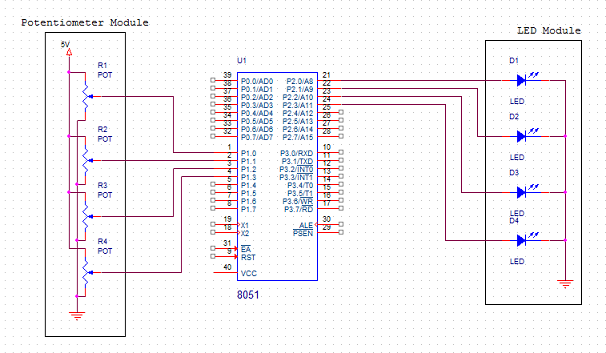
\includegraphics[width=\textwidth]{Schematic.png}
		\caption{Circuit schematic for lab}
		\label{schematic}
	\end{figure}
\pagebreak
\subsection{Part 1}
\subsubsection{Code}
	\lstinputlisting{part1_publish.c}
\subsection{Part 2}
\subsubsection{Code}
	\lstinputlisting{part2_publish.c}	
\subsection{Part 3}
\subsubsection{Code}
	\lstinputlisting{part3_publish.c}
\subsection{Enhancement}
\subsubsection{Code}
	\lstinputlisting{encahncement.c}

\section{References} 
\noindent
``MPS Lab 5," in RPI ECSE Department, 2016. [Online]. Available: \url{http://www.rpi.edu/dept/ecse/mps/MPS_Lab_Ex5-Memory.pdf}. Accessed: Nov. 13, 2016.\\
\newline\noindent
``C8051 Manual," in RPI ECSE Department, 1.4 ed., 2005. [Online]. Available: \url{https://www.ecse.rpi.edu/courses/CStudio/Silabs/C8051F12x-13x.pdf}. Accessed: Nov. 13, 2016.


\end{document}